\subsubsection{Anwendungsszenario}
Dieser Abschnitt beschreibt die Anforderungen an das Softwaresystem mittels Anwendungsfällen und 
beschreibt die technischen Rahmenbedingungen, in dem das Softwaresystem eingebettet ist.
\subsubsection{Use Cases}

Die Anwendungsfälle beschreiben die Arbeit mit dem \textit{One-Million-Song}-Datensatz. 

Das Anwendungsfalldiagramm \ref{anforderungen:usecasediagramm} zeigt alle Anwendungsfälle für
die Arbeit mit dem Million-Song-Datensatz auf dem Hochschul-Cluster.

\begin{figure}[H]
	\centering
	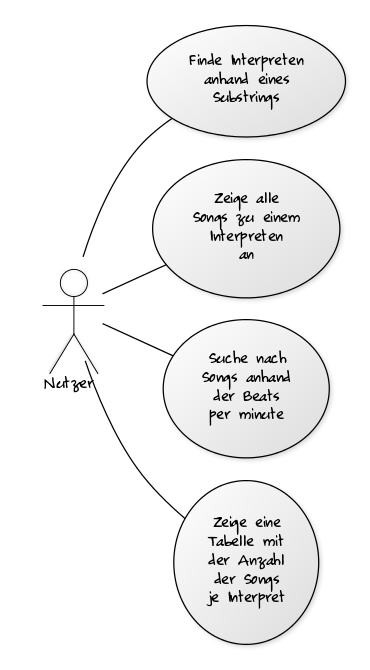
\includegraphics[width=0.5\textwidth]{images/06usecases.png}
	\caption{Anwendungsfall-Diagramm, UML 2.0. Alle Anwendungsfälle für das Million-Song-Projekt}
	\label{anforderungen:usecasediagramm}
\end{figure}

Es folgt eine kurze Beschreibung der einzelnen Anwendungsfälle. Auf eine detaillierte Ausarbeitung im Rahmen einer 
ausführlichen Anforderungsanalyse soll in diesem Falle verzichtet werden, weil ein konkretes Anwendungsszenario fehlt und
die Anwendungsfälle künstlicher Natur sind, um den Einsatz von Hadoop, MapReduce und Hbase im Bereich einer
Big-Data-Anwendung zu evaluieren.

\begin{description}
	\item[UC 1] Der Nutzer möchte eine Motto-Party veranstalten. Er kann sich allerdings nicht mehr genau an den Namen des Interpreten erinnern. Mit Hilfe der Vorschläge, die ihm dynamisch während des Tippens angezeigt werden, ist es ihm möglich den Interpreten zu finden.
	\item[UC 2] Der Nutzer möchte nun alle Songs zu einem Interpreten aus \textbf{UC 1} anzeigen.
	\item[UC 3] Der Nutzer möchte ein speziell für ihn angepasstes Lauftraining absolvieren. Dazu sucht er nach Songs mit einer speziellen \ac{BPM}-Rate.
	\item[UC 4] Der Nutzer möchte nach besonders erfolgreichen Interpreten in der Datenbank suchen. Daher lässt er sich eine Tabelle ausgeben, in der die Songs pro Interpret dargestellt werden.

\end{description}

\subsubsection{Parametriesierbarkeit}
\label{anforderungen:rahmenbedingungen}
Die Rahmenbedingungen teilen sich in die Hardware-Rahmenbedingungen und in die Software-Rahmenbedingungen auf.
Die Hardware, die uns zur Verfügung gestellt wurde besteht aus einem Verbund von 5 homogenen Server-Rechnern, 
die über ein Ethernet-Netzwerk gleichwertig miteinander verknüpft sind. Physikalisch sind alle Knoten an einem gemeinsamen
Switch angeschlossen als physikalische Stern-Topologie. Dies hat aus logischer Sicht zur Folge, dass eine direkte Kommunikation
zwischen den Knoten möglich ist. Die Bandbreite des gesamten Netzwerkes ist mit 20Mbit/s angegeben, was durch die Topologie
auch zwischen den einzelnen Knoten möglich wäre.

Die Server-Knoten sind alle mit folgender Hardware ausgestattet:
\begin{itemize}
	\item Intel i7-4790K CPU
	\item 32 GB RAM
	\item 256 GB SSD
	\item 2 TB HDD
\end{itemize}

Auf der Seite der Software ist auf allen Knoten mit \textit{Ubuntu} eine Linux-Distribution in der Version 
\textit{16.04.1 LTS Server 64-Bit} installiert. Root-Rechte sind gewährt.
Anzumerken ist, dass alle Ressourcen mit 9 anderen Teams geteilt werden und alle Teams auf der selben 
Instanz des Betriebssystems arbeiten und nur durch unterschiedliche Nutzer getrennt sind. 
Diese Rahmenbedingung ist insbesondere bei der Konfiguration der Netzwerk-Ports bei verteilten Anwendungen 
zu beachten, da verschiedene Anwendungen eventuell auf dem gleichen Port lauschen und somit 
Konflikte entstehen können.

\subsubsection{Installation und Konfiguration}
Auf dem Cluster wird das komplette Hadoop-Softwarepaket installiert, bestehend aus den
Komponenten \ac{YARN}, \ac{HDFS} und MapReduce. Installiert wird über einen Tarball von der offiziellen
Apache-Webseite (\url{http://www-us.apache.org/dist/hadoop/common/hadoop-2.7.3/hadoop-2.7.3.tar.gz}), um die aktuellste Version ($2.7.3$) von Hadoop zu erhalten. Die Installation selbst gestaltet sich mit dem Entpacken der Binär-Dateien im home-Verzeichnis 
denkbar einfach. Komplexer gestaltet sich die Konfiguration, die das Laufzeitverhalten der Komponenten festlegen.

Die folgenden Tabellen zeigen die Konfiguration der einzelnen Hadoop-Komponenten, die vom Standard abweicht.
Eine Auflistung der ab Werk ausgelieferten Standard-Konfiguration kann auf folgenden Webseiten nachgeschlagen werden:
\cite{hdfsDefault}, \cite{yarnDefault}, \cite{mapreduceDefault} \cite{hbaseConfig}.

Tabellen zeigen die Konfiguration von HDFS \ref{config:hdfsValues}, YARN \ref{config:yarnValues}, MapReduce \ref{config:mapreduceValues} und HBase 
speziell für die vorhandene Cluster-Umgebung. Es werden  nur Parameter aufgelistet, 
die von der Werks-Konfiguration abweichen.
Hbase liefert von Haus aus bereits eine eigene ZooKeeper-Installation mit. Der Grund für eine eigene, getrennte ZooKeeper-Installation lag in der sauberen Trennung zwischen der Hbase-Konfiguration und der ZooKeeper-Konfiguration. 

\subsubsection{Berechnung der Speicher-Konfiguration}
\label{anforderung:berechungSpeicher}
Im Zuge der Probleme mit der Ausführung einer Map-Reduce-Jobs, bei dem die Rechnerknoten
offenbar wegen Überlastung ihren Dienst quittierten, wird die Speicher-Verwendung
des Map-Reduce-Frameworks manuell eingestellt. Der Algorithmus zur Berechnung der 
benötigen Speichermengen ist \cite{memoryCal} Unterpunkt \textit{ 10.2. Manually Calculating YARN and MapReduce Memory Configuration Settings} entnommen.
Grundlage für die Berechnung ist die verfügbare Hardware auf den Rechnerknoten, speziell
die verfügbare Menge an Speicher, die Anzahl an Prozessor-Kernen und die Anzahl an 
Festplatten. Basierend auf der gegebenen Hardware-Spezifikation des Clusters 
(siehe \ref{anforderungen:rahmenbedingungen}) ergaben sich die Grund-Parameter in Tabelle
\ref{config:memoryCalculation}.
Dabei wurde der verfügbare Speicher von 32 auf 8 GB gekürzt, um die Speichernutzung der
anderen Teams auf dem Cluster zu berücksichtigen.

\begin{table}
	\begin{tabularx}{\textwidth}{|X|X|} \hline
	Speicher & 8 GB \\ \hline
	Kerne & 8 \\ \hline
	Festplatten & 1 \\ \hline
	\end{tabularx}
	\caption{Grund-Parameter zur Berechnung der Map-Reduce Speicherverwendung}
	\label{config:memoryCalculation}
\end{table}

Als Zwischen-Ergebnis der Berechnung erhält man die maximale Anzahl an parallel laufenden 
Containern pro Rechnerknoten und der die Menge an Speicher pro Container. Für dieses Cluster
ergibt die Berechnung eine Container-Anzahl von $3$ maximal parallelen Containern und 
eine empfohlene Zuweisung von $1536$ Megabyte pro Container. Mit diesen Parametern lässt 
sich nun die empfohlene Speicher-Konfiguration des Map-Reduce-Frameworks berechnen, die
weiter oben als Konfiguration in den Tabellen \ref{config:yarnDescription} und
 \ref{config:mapreduceValues} zu sehen ist.